\documentclass[a4paper,12pt]{article}

\usepackage{geometry}
\usepackage{fontspec}
\usepackage{listings}
\usepackage{xcolor}
\usepackage{enumitem}
\usepackage{hyperref}
\usepackage{graphicx}
\usepackage{caption}
\usepackage{fancyhdr}
\usepackage{calc}

\geometry{margin=25mm}
\pagestyle{fancy}
\hbadness=10000
\fancyhf{}
\fancyfoot[R]{\small\thepage}
\renewcommand{\headrulewidth}{0pt}
\renewcommand{\footrulewidth}{0pt}
\captionsetup{font=small, labelfont=bf, textfont=it}

\setmainfont{InterDisplay}[
  UprightFont=*-Regular,
  ItalicFont=*-Italic,
  BoldFont=*-Bold,
  BoldItalicFont=*-BoldItalic,
  FontFace={ul}{n}{Font={*-Thin}},
  FontFace={ul}{it}{Font={*-ThinItalic}},
  FontFace={el}{n}{Font={*-ExtraLight}},
  FontFace={el}{it}{Font={*-ExtraLightItalic}},
  FontFace={l}{n}{Font={*-Light}},
  FontFace={l}{it}{Font={*-LightItalic}},
  FontFace={mb}{n}{Font={*-Medium}},
  FontFace={mb}{it}{Font={*-MediumItalic}},
  FontFace={sb}{n}{Font={*-SemiBold}},
  FontFace={sb}{it}{Font={*-SemiBoldItalic}},
  FontFace={eb}{n}{Font={*-ExtraBold}},
  FontFace={eb}{it}{Font={*-ExtraBoldItalic}},
  FontFace={ub}{n}{Font={*-Black}},
  FontFace={ub}{it}{Font={*-BlackItalic}},
  RawFeature={+cv05}
]
\setmonofont{Adwaita Mono}
\DeclareRobustCommand{\regular}{\fontseries{m}\selectfont}
\DeclareRobustCommand{\medium}{\fontseries{mb}\selectfont}
\DeclareRobustCommand{\sbold}{\fontseries{sb}\selectfont}
\DeclareRobustCommand{\bold}{\fontseries{b}\selectfont}
\renewcommand{\small}{\fontsize{10}{12}\selectfont}
\newcommand{\rcode}[1]{\texttt{\fontsize{11}{13}\selectfont#1}}
\newcommand{\bcode}[1]{\texttt{\fontsize{11}{13}\selectfont\bold#1}}

\lstset{
    basicstyle = {\small\ttfamily},
    breaklines = true,
    columns = fullflexible,
    keepspaces = true,
    aboveskip = 0mm,
    belowskip = 0mm,
    showstringspaces = false,
    numbers = left,
    numberstyle = \small\ttfamily,
    numbersep = 2.5mm,
    xleftmargin = 6.5mm
}

% Title
\title{\vspace{-25mm}{\normalsize\addfontfeatures{
  RawFeature={+cv08}}Semester I 2025}\\{
  \large\addfontfeatures{RawFeature={+cv08}}\medium{
  Astroinformatics I}}\\\LARGE\sbold{Graded Practice 3}}
\author{}
\date{\vspace{-22.5mm}}

% Set indent to 5mm
\setlist[enumerate,1]{left=0mm, labelsep=2.5mm, itemsep = \baselineskip,
topsep = \baselineskip}
\setlist[enumerate,2]{left=-1mm, labelsep=2.5mm}
\newenvironment{solution}{}{}

\begin{document}
\maketitle
\thispagestyle{fancy}
\sbold{\hspace{-6mm}José B. Batista M.\\}
\begin{enumerate}
  \item Repeat the plots from graded practice 1, but now with Python using the
  light curve filesfrom practice 2. For the plots, take into account how to make
  them more readable.
  \begin{solution}
    \\\\\regular The Python script snippet provided below (saved as
    \bcode{practice\_3.py}) generates raw light curve plots for each light curve
    file present in the \bcode{lc\_data\_folder} directory. The \bcode{get\_lc\_data}
    function is used to load and preprocess the TESS light curve files into an
    Astropy \bcode{TimeSeries} object. This function reads a light curve file,
    parses its columns (\bcode{TIME}, \bcode{PDCSAP\_FLUX}, and \bcode{PDCSAP\_FLUX\_ERR}),
    and converts times to JD in TDB scale. It also converts each BJD timestamp
    to a UTC calendar date string, which is included as a new column, to be used.
    in the plots. The \bcode{plot\_raw\_lc} function is responsible for creating
    these plots. It uses \bcode{matplotlib} to generate scatter plots with error
    bars for flux values against BJD Epoch. To enhance readability and accessibility,
    the script utilizes different markers and a colorblind-fiendly palette for
    data points corresponding to unique observation dates (taken from the date
    string column). A legend is included to distinguish the dates, and axis labels
    and a title are provided for clarity. The plots are saved as PDF files in the
    \bcode{Plots} directory.\\
\begin{lstlisting}[language=Python]
import os, itertools, numpy as np, matplotlib.pyplot as plt, pandas as pd
from astropy.time import Time
from astropy.timeseries import TimeSeries, LombScargle
from astropy import units as u

lc_data_folder = 'Practices/Practice_3/LC_Files'

def get_lc_data(filename):
    '''
    Load and preprocess a TESS light curve file into an Astropy TimeSeries object.
    
    This function reads a light curve file from the specified folder, parses its
    columns (BTJD time, PDCSAP_FLUX, and flux error), and converts times to JD
    in TDB scale. It also converts each BJD timestamp to a UTC calendar date
    string, which is included as a new column.
    
    Parameters
    ----------
    filename : str
        The name of the light curve file (relative to `lc_data_folder`).
    
    
    Returns
    -------
    lc_data : astropy.timeseries.TimeSeries
        A TimeSeries object with columns:
        - time (BJD, TDB)
        - flux (in e-/s)
        - flux_err (in e-/s)
        - date (UTC calendar date string in 'YYYY-MM-DD' format)
    
    Raises
    ------
    FileNotFoundError
        If the specified file does not exist in the data folder.
    Exception
        For any other parsing or conversion errors.
    '''
    try:
        lc_file = os.path.join(lc_data_folder, filename)
        lc_df = pd.read_csv(lc_file, sep=' ', skiprows = 1, names=['TIME',
                            'PDCSAP_FLUX', 'PDCSAP_FLUX_ERR'])
        lc_df = lc_df.dropna()
        btjd = lc_df['TIME'].astype(float)
        flux = lc_df['PDCSAP_FLUX'].astype(float)
        flux_error = lc_df['PDCSAP_FLUX_ERR'].astype(float)
        bjd = btjd + 2457000.0
        bjd_epoch = Time(bjd, format = 'jd', scale = 'tdb')
        dates_utc = bjd_epoch.utc.datetime
        date_strs = [date.strftime('%Y-%m-%d') for date in dates_utc]
        lc_df['DATE'] = date_strs
        lc_data = TimeSeries(time=bjd_epoch,
                             data={'flux': flux * u.electron/u.s,
                                   'flux_err': flux_error * u.electron/u.s,
                                   'date': lc_df['DATE'].values})
        return lc_data
    except FileNotFoundError:
        print(f'Error: File not found at {filename}')
        exit()
    except Exception as e:
        print(f'An error occurred while loading the file: {e}')
        exit()

def plot_raw_lc(filename, lc_data):
    '''
    Plot the raw light curve with flux grouped by observation date.

    This function generates a scatter plot of a light curve with error bars, grouping points
    by date using distinct marker/colour combinations. The figure is saved to a PDF file.

    Parameters
    ----------
    filename : str
        Name of the light curve file being processed. Used for the plot title and output filename.
    lc_data : astropy.timeseries.TimeSeries
        Light curve time series object containing 'time', 'flux', 'flux_err', and 'date' columns.

    Notes
    -----
    - The plot legend is arranged in multiple columns below the plot to avoid overlapping data.
    - The output plot is saved as a PDF in the `Practices/Practice_3/Plots/` directory.
    '''
    #plt.rc('xtick', labelsize='x-small')
    #plt.rc('ytick', labelsize='x-small')
    plt.figure(figsize=(10, 6))
    colors = ['#E69F00', '#0077FF', 'w','gray']
    shapes = ['o', 's', '^', 'D', 'v', '<', '>', 'P', '*', 'h', 'd', 'p']
    markers = list(itertools.product(shapes, colors))
    unique_dates = np.unique(lc_data['date'])
    num_labels = len(unique_dates)
    n_cols = int(np.ceil(num_labels/3))
    for i, date in enumerate(unique_dates):
        mask = lc_data['date'] == date
        marker = markers[i % len(markers)]
        shape, color = marker
        plt.errorbar(lc_data.time[mask].value, lc_data['flux'][mask].value,
                     yerr=lc_data['flux_err'][mask].value, fmt=shape,
                     color=color, ms=4, markeredgecolor='k', markeredgewidth=0.5,
                     alpha=0.75, label=f'{date}')
    plt.xlabel('BJD Epoch')
    plt.ylabel(r'PDCSAP Flux (e$^{{-}}$/s)')
    plt.title(f'Lightcurve of {filename}')
    plt.legend(fontsize='small', ncol=n_cols, loc='upper center',
               bbox_to_anchor=(0.5, -0.1), fancybox=True, shadow=True)
    plt.tight_layout()
    plt.savefig(f'Practices/Practice_3/Plots/{filename}_raw.pdf',
                format='pdf')
    plt.close()

for filename in os.listdir(lc_data_folder):
    lc_data = get_lc_data(filename)
    plot_raw_lc(filename, lc_data)\end{lstlisting}
  \vspace{1em}One of the resulting light curve plots is shown below (all plots
  for this practice, as well as the Python script, are available in a
  \href{https://github.com/josebatistam/Astroinformatics_I}{repository}).\pagebreak
  \begin{figure}[htbp]
    \centering
    \hspace{5mm}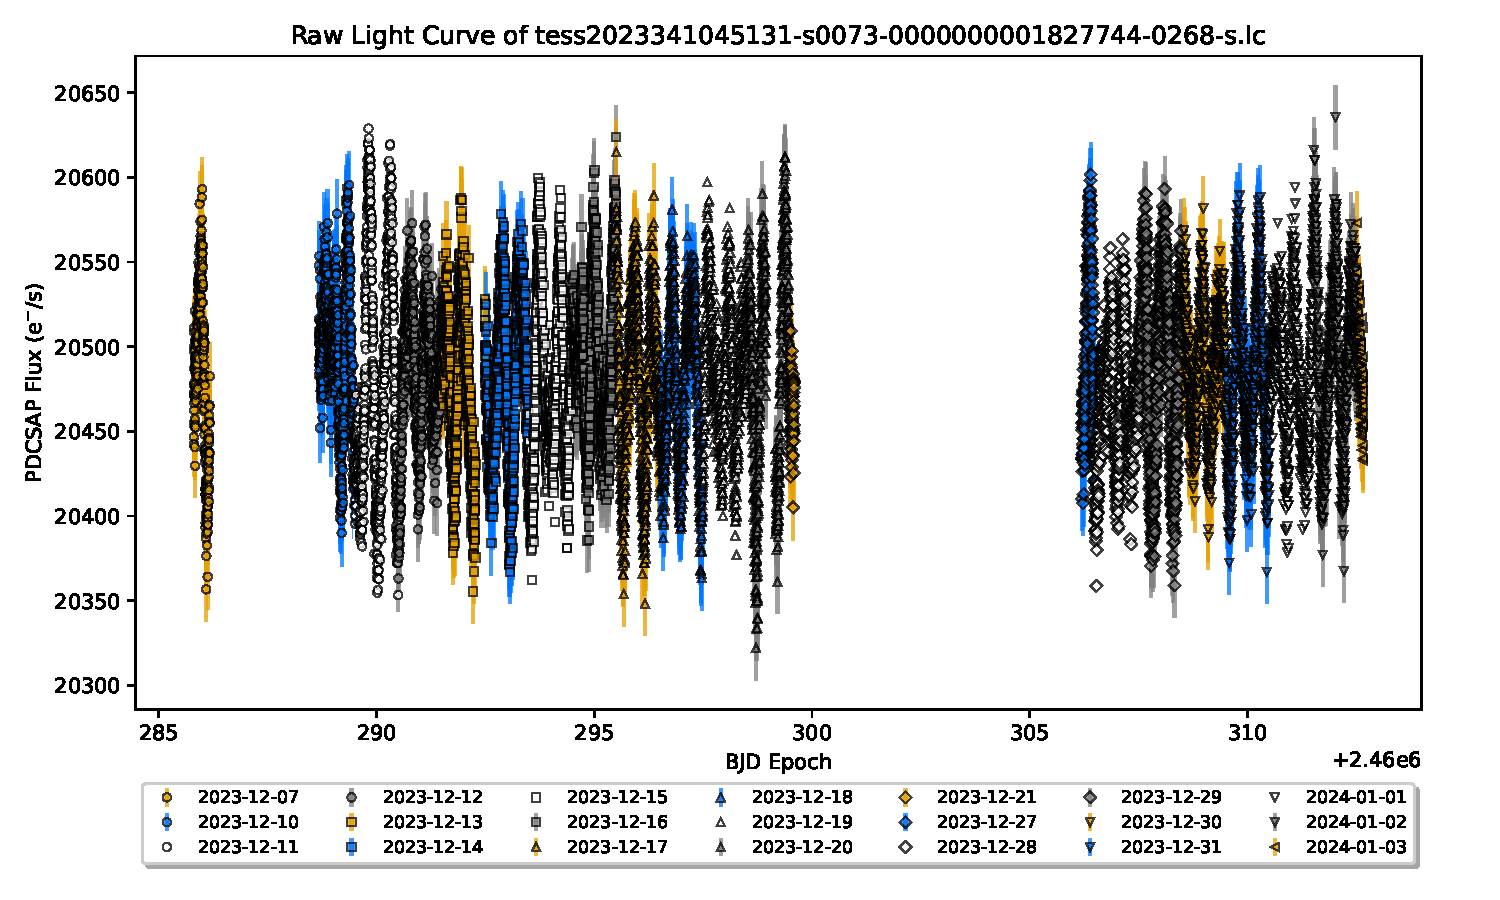
\includegraphics[width = 1\textwidth]{
      ../Plots/tess2023341045131-s0073-0000000001827744-0268-s.lc_raw_1.pdf}
  \end{figure}
  \end{solution}\vspace{-1em}
  \item When you make the plots, can you identify outliers? Highlight them. Try
  writing code to identify at least the most extreme outliers.
  \begin{solution}
    \\\\\regular The Python script snipped provided below identifies and highlights
    outliers in the raw light curve plots. The \bcode{identify\_outliers} function
    performs a robust sigma-clipping method to detect outliers. For each unique
    observing date, it calculates the median and median absolute deviation (mad)
    of the flux values. Points deviating more than a specified threshold
    (defaulting to 3) times the robust sigma estimate (\bcode{1.4826*mad}) are
    flagged as outliers. These identified outliers are then plotted with a distinct
    black \bcode{'x'} marker on the raw light curve plots, making them clearly
    visible.\\
    \begin{lstlisting}[language=python]
def identify_outliers(flux, dates, threshold=3):
    '''
    Identify outliers in a light curve using robust sigma-clipping per observing
    date.

    For each unique date, this function computes the median and MAD (median
    absolute deviation) of the flux values, then flags as outliers all points 
    deviating more than `threshold` times the robust sigma estimate.

    Parameters
    ----------
    flux : ndarray
        Array of flux values (e.g., in e-/s).
    dates : array-like of str
        Array of corresponding unique date strings in 'YYYY-MM-DD' format, one
        per flux value.
    threshold : float, optional
        Number of robust standard deviations (sigma) to use for outlier rejection.
        Default is 3.

    Returns
    -------
    outlier_mask : ndarray of bool
        Boolean array of the same length as `flux`, where `True` marks an outlier.
    '''
    outlier_mask = np.zeros(len(flux), dtype=bool)
    for date in dates:
        mask = dates == date
        flux_day = flux[mask]
        median = np.median(flux_day)
        mad = np.median(np.abs(flux_day - median))
        sigma = 1.4826 * mad
        outliers = np.abs(flux_day - median) > threshold * sigma
        outlier_mask[mask] = outliers
    return outlier_mask

# ---- UPDATED PLOT FUNCTION -----

def plot_raw_lc(filename, lc_data, threshold=3):
    '''
    Plot the raw light curve with flux grouped by observation date and annotated outliers.

    This function generates a scatter plot of a light curve with error bars, grouping points
    by date using distinct marker/colour combinations. Outliers are identified using
    sigma-clipping and plotted with a distinct marker. The figure is saved to a PDF file.

    Parameters
    ----------
    filename : str
        Name of the light curve file being processed. Used for the plot title and output filename.
    lc_data : astropy.timeseries.TimeSeries
        Light curve time series object containing 'time', 'flux', 'flux_err', and 'date' columns.
    threshold : float, optional
        Sigma threshold for outlier rejection (default is 3).
    
    Notes
    -----
    - Outliers are identified per date using the `identify_outliers` function with a default
      threshold of 3σ.
    - The plot legend is arranged in multiple columns below the plot to avoid overlapping data.
    - The output plot is saved as a PDF in the `Practices/Practice_3/Plots/` directory.
    '''
    #plt.rc('xtick', labelsize='x-small')
    #plt.rc('ytick', labelsize='x-small')
    plt.figure(figsize=(10, 6))
    colors = ['#E69F00', '#0077FF', 'w','gray']
    shapes = ['o', 's', '^', 'D', 'v', '<', '>', 'P', '*', 'h', 'd', 'p']
    markers = list(itertools.product(shapes, colors))
    unique_dates = np.unique(lc_data['date'])
    flux = lc_data['flux'].value
    dates = lc_data['date']
    outlier_mask = identify_outliers(flux, dates, threshold)
    num_labels = len(unique_dates)
    n_cols = int(np.ceil(num_labels/3))
    for i, date in enumerate(unique_dates):
        mask = lc_data['date'] == date
        marker = markers[i % len(markers)]
        shape, color = marker
        plt.errorbar(lc_data.time[mask].value, lc_data['flux'][mask].value,
                     yerr=lc_data['flux_err'][mask].value, fmt=shape,
                     color=color, ms=4, markeredgecolor='k', markeredgewidth=0.5,
                     alpha=0.75, label=f'{date}')
    plt.scatter(lc_data.time[outlier_mask].value,
                lc_data['flux'][outlier_mask].value, marker='x', color='k', s=25,
                label = fr'{threshold}$\sigma$ Outliers', zorder=10)
    plt.xlabel('BJD Epoch')
    plt.ylabel(r'PDCSAP Flux (e$^{{-}}$/s)')
    plt.title(f'Raw Light Curve of {filename}')
    plt.legend(fontsize='small', ncol=n_cols, loc='upper center',
               bbox_to_anchor=(0.5, -0.1), fancybox=True, shadow=True)
    plt.tight_layout()
    plt.savefig(f'Practices/Practice_3/Plots/{filename}_raw.pdf',
                format='pdf')
    plt.close()

outliers_sigma = 3
for filename in os.listdir(lc_data_folder):
    lc_data = get_lc_data(filename)
    plot_raw_lc(filename, lc_data, outliers_sigma)\end{lstlisting}
  \vspace{1em} The updated light curve plot with the highlighted outliers for
  the same example is shown in the figure below.\pagebreak
  \begin{figure}[htbp]
    \centering
    \hspace{5mm}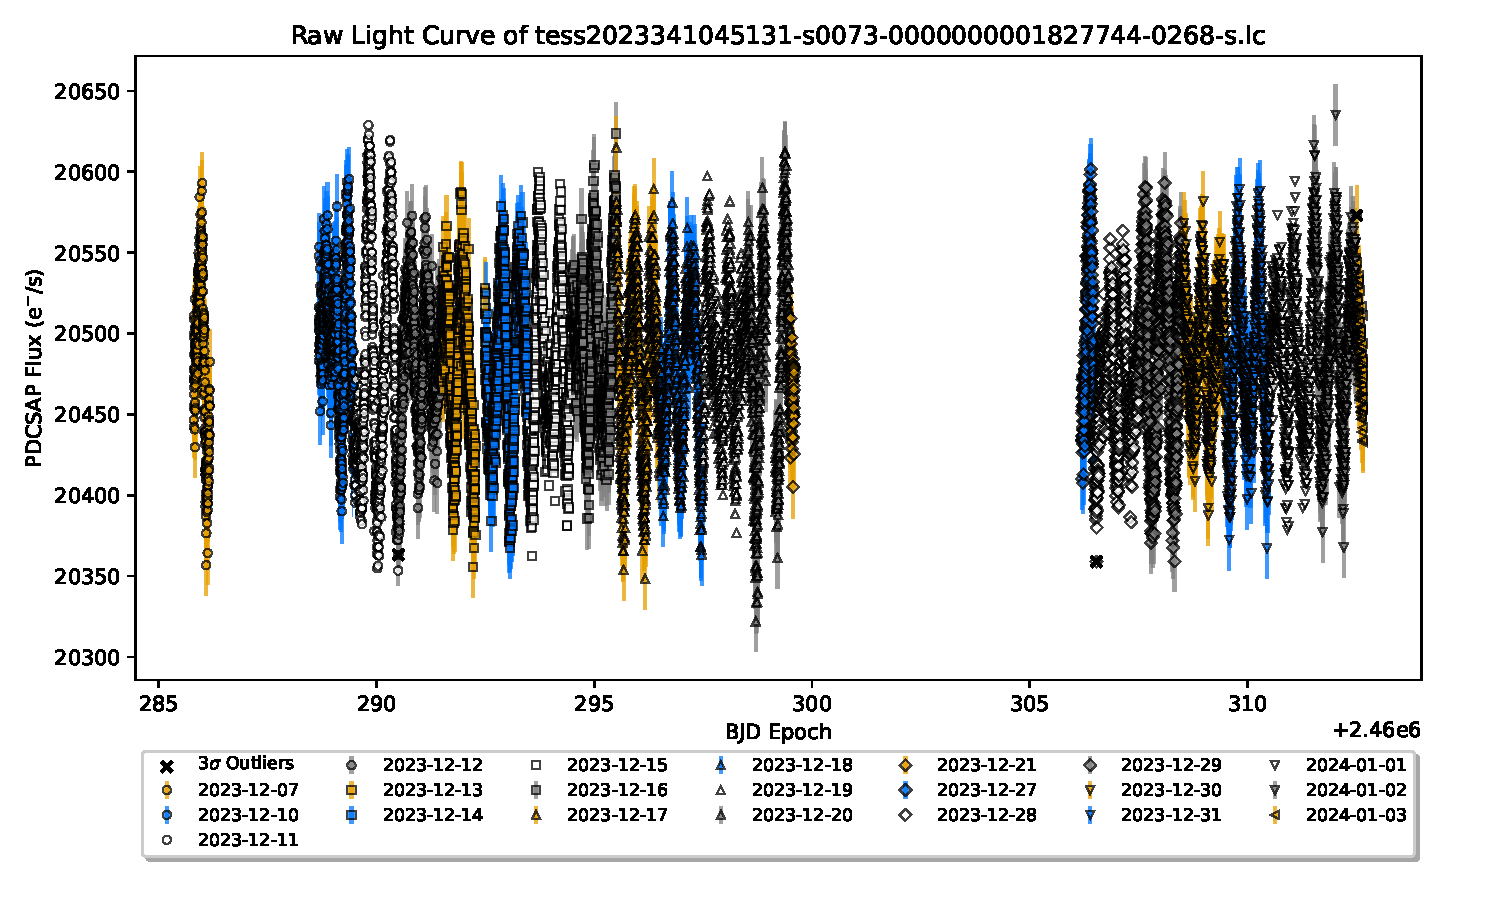
\includegraphics[width = 1\textwidth]{
      ../Plots/tess2023341045131-s0073-0000000001827744-0268-s.lc_raw.pdf}
  \end{figure}
  \end{solution}\vspace{-1em}
  \item Think about basic statistics to describe light curves, such as amplitudes,
  and implementat least two of them.
  \begin{solution}
    \\\\\regular The Python script snippet provided below mplements basic statistics
    to describe light curves, specifically focusing on the phase, period and
    amplitude. The \bcode{fold\_lc} function analyzes and plots a phase-folded
    light curve and its Lomb-Scargle periodogram. It first prepares the data by
    masking out outliers using the \bcode{identify\_outliers} function with the
    specified threshold. It then computes the Lomb-Scargle periodogram to find
    the best period within a given range (\bcode{min\_period} to \bcode{max\_period}).
    The light curve is then phase-folded using this best period. Finally, the
    amplitude is estimated from the folded light curve as the difference between
    the 97.5th and 2.5th percentiles of the flux values. The function generates
    a two-subplot figure, displaying both the phase-folded light curve and the
    Lomb-Scargle periodogram, along with annotations for the period, amplitude,
    and an estimated initial BJD epoch.\\
    \begin{lstlisting}[language=python]
def fold_lc(filename, lc_data, threshold=3, min_period=0.1, max_period=10):
    """
    Analyse and plot a phase-folded light curve and its Lomb-Scargle periodogram.

    Parameters
    ----------
    lc_data : astropy.timeseries.TimeSeries
        Light curve data with 'time', 'flux', 'flux_err', and 'date' columns.
    filename : str
        Filename for plot titles.
    threshold : float, optional
        Sigma threshold for outlier rejection (default is 3).
    min_period : float, optional
        Minimum period to search (days), default 0.1.
    max_period : float, optional
        Maximum period to search (days), default 10.
    """
    # Prepare data and mask out outliers
    flux = lc_data['flux'].value
    flux_err = lc_data['flux_err'].value
    dates = lc_data['date']
    time = lc_data.time.value
    mask = ~identify_outliers(flux, dates, threshold)
    time_clean = time[mask]
    flux_clean = flux[mask]
    flux_err_clean = flux_err[mask]
    dates_clean = dates[mask]
    bjd_0 = np.median(time_clean)
    # Compute Lomb-Scargle periodogram
    ls = LombScargle(time_clean, flux_clean, flux_err_clean)
    frequency, power = ls.autopower(minimum_frequency=1/max_period,
                                    maximum_frequency=1/min_period,
                                    samples_per_peak = 25)
    best_frequency = frequency[np.argmax(power)]
    best_period = 1 / best_frequency
    # Phase folding
    phase = (time_clean % best_period) / best_period
    # Estimate amplitude from folded light curve
    amplitude = np.percentile(flux_clean, 97.5) - np.percentile(flux_clean, 2.5)
    # Create figure with two subplots (folded LC + periodogram)
    fig, (ax1, ax2) = plt.subplots(2, 1, figsize=(10, 8),
                                   gridspec_kw={'height_ratios': [2, 1]})
    # Plot folded light curve
    shapes = ['o', 's', '^', 'D', 'v', '<', '>', 'P', '*', 'h', 'd', 'p']
    colors = ['orange', "#0050FF", 'w', 'gray']
    markers = list(itertools.product(shapes, colors))
    unique_dates = np.unique(dates_clean)
    n_cols = int(np.ceil(len(unique_dates) / 3))
    for i, date in enumerate(unique_dates):
        mask_date = dates_clean == date
        shape, color = markers[i % len(markers)]
        ax1.errorbar(phase[mask_date], flux_clean[mask_date],
                     yerr=flux_err_clean[mask_date], fmt=shape, color=color,
                     ms=4, alpha=0.75, markeredgecolor='k', markeredgewidth=0.5,
                     label=date)
    ax1.set_xlabel('Phase')
    ax1.set_ylabel(r'PDCSAP Flux (e$^{{-}}$/s)')
    ax1.set_title(f'Phase-Folded Light Curve of {filename}')
    # Annotation above x-axis in the folded plot
    info_text = rf'$BJD_0$: {bjd_0},$\quad$Period: {best_period:.5f} d,$\quad$Amplitude: $\sim${amplitude:.2f} e$^{{-}}$/s'
    ax1.annotate(
        info_text,
        xy = (0.01, 0.01),
        xycoords = 'axes fraction',
        fontsize = 9,
        color = 'black',
    )
    ax1.legend(fontsize='small', ncol=n_cols, loc='upper center',
               bbox_to_anchor=(0.5, -0.1), fancybox=True, shadow=True)
    # Plot periodogram
    ax2.plot(1/frequency, power, color="#0050FF")
    max_power = np.max(power)
    ax2.annotate(
        f'Best Period: {best_period:.5f} d',
        xy = (best_period, max_power),
        xytext = (best_period + 0.15*(max_period - best_period), 0.8*max_power),
        arrowprops = dict(shrink=0.1, width=1.5, headwidth=5, facecolor='orange',
                          edgecolor = 'none'),
        ha = 'center',
        color = 'k',
        fontsize = 9
    )
    ax2.set_xlabel('Period (days)')
    ax2.set_ylabel('Lomb-Scargle Power')
    ax2.set_title('Lomb-Scargle Periodogram')
    plt.tight_layout()
    plt.savefig(f'Practices/Practice_3/Plots/{filename}_folded.pdf',
                format='pdf')
    plt.close()

outliers_sigma = 3
for filename in os.listdir(lc_data_folder):
    lc_data = get_lc_data(filename)
    fold_lc(filename, lc_data, threshold=outliers_sigma)\end{lstlisting}
  \vspace{1em} The folded light curve plot with the periodogram for the same
  example is shown in the figure below.
  \\\\It's important to note that not all light curves fold as well as the example
  shown. The periodogram of most of the light curves have spurious peaks, which
  could be due to several factors such as dropping \bcode{NaN} values from the data,
  gaps in the TESS observations, the signal not beign a perfect sinusoid, the
  presence of aliases due to the observation setup, etc. The interaction of these
  (and other) effects means that in practice there is no absolute guarantee that
  the highest peak corresponds to the best frequency, and results must be
  interpreted carefully.\pagebreak
  \begin{figure}[htbp]
    \centering
    \hspace{5mm}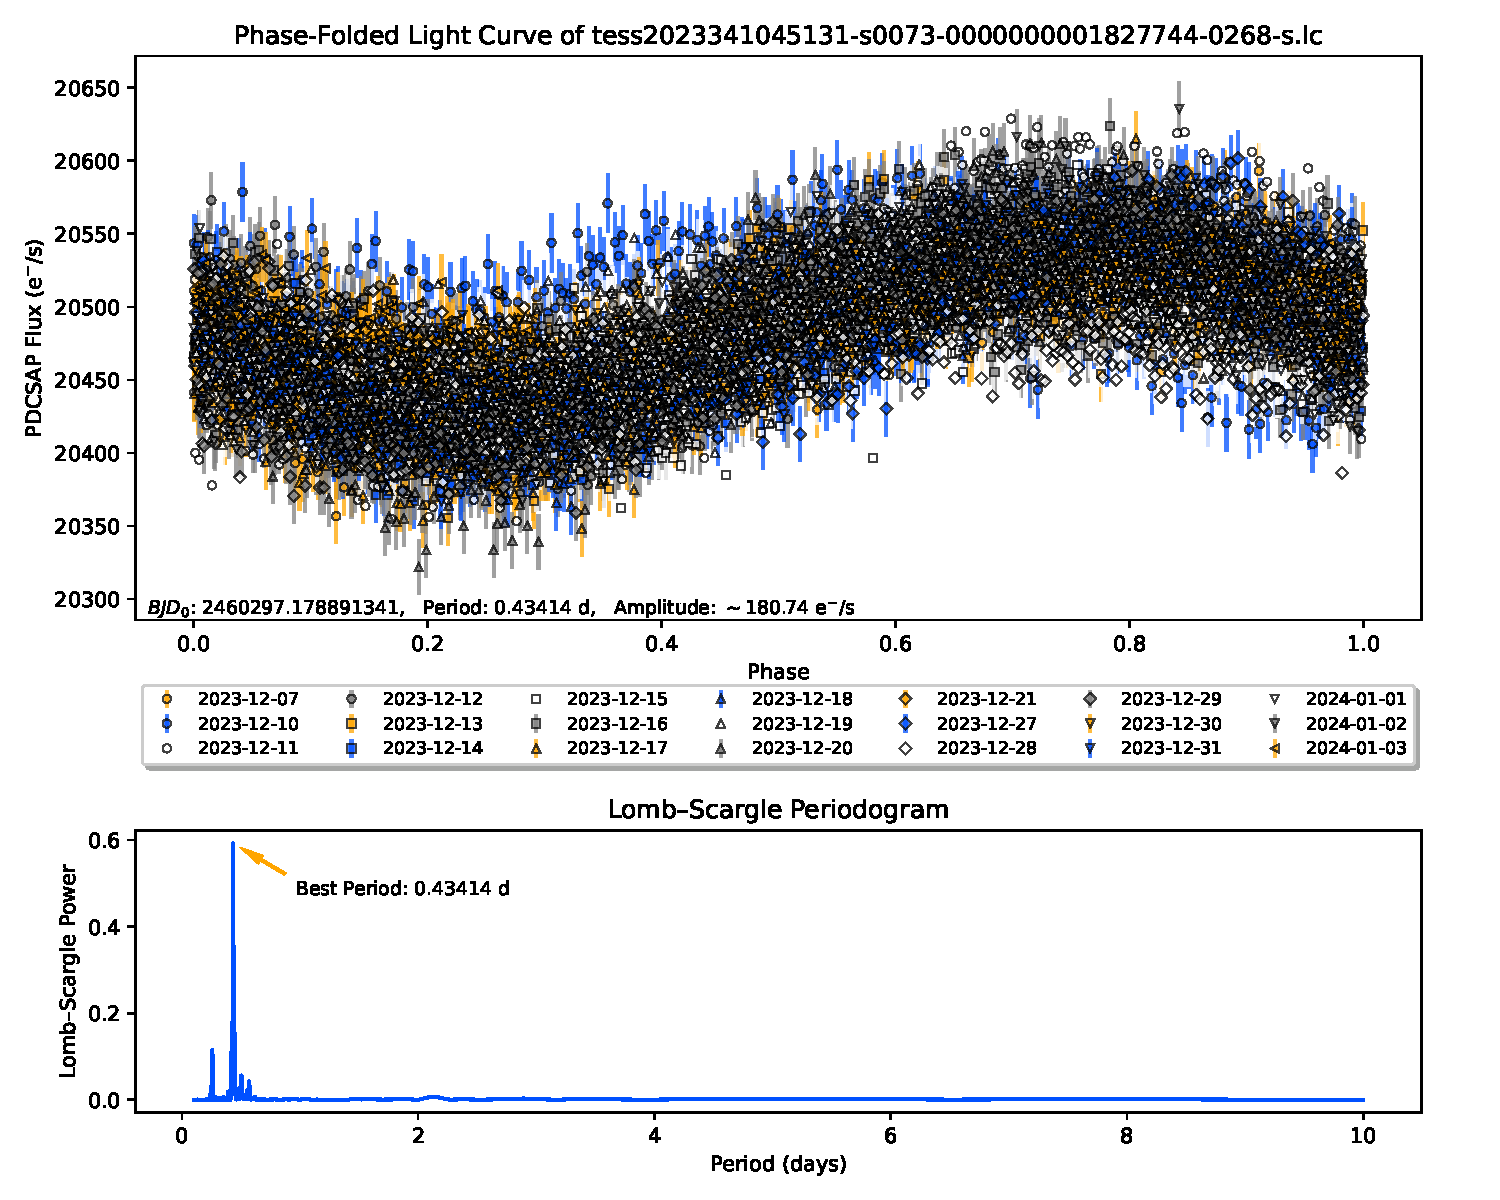
\includegraphics[width = 1\textwidth]{
      ../Plots/tess2023341045131-s0073-0000000001827744-0268-s.lc_folded.pdf}
  \end{figure}
  \end{solution}
\end{enumerate}
\end{document}